\documentclass[aps,prb,twocolumn,
	groupedaddress,superscriptaddress,
	amsfonts,amssymb,amsmath,floatfix,
	citeautoscript]{revtex4-1}

\usepackage{graphicx}
\usepackage[centering,hmargin=20mm,tmargin=30mm,bmargin=25mm]{geometry}
\usepackage{multirow}
\usepackage{newtxtext}
\usepackage[cmintegrals]{newtxmath}

%----- References -----
\usepackage{xcolor}
\usepackage{hyperref}
\hypersetup{colorlinks,
	linkcolor={blue!75!black!80!yellow},
	citecolor={blue!75!black!80!yellow},
	urlcolor={blue!75!black!80!yellow}
}

%----- Captions in sans font -----
\makeatletter
\renewcommand\@make@capt@title[2]{%
	\@ifx@empty\float@link{\@firstofone}{\expandafter\href\expandafter{\float@link}}%
	\sffamily{\textbf{#1}}\@caption@fignum@sep#2
}%
\renewcommand\figurename{Fig.}
\makeatother

\thickmuskip=5mu plus 2mu minus 1mu  %binary relations (default, 5mu plus 5mu)
\medmuskip=4mu plus 2mu minus 2mu    %binary operations (default, 4mu plus 2mu minus 4mu)

\frenchspacing %Ensure that revTeX does not do "double spaces" after punctuation

\renewcommand{\Im}{\operatorname{Im}}
\renewcommand{\Re}{\operatorname{Re}}
\newcommand{\sub}[1]{\ensuremath{_{\textrm{#1}}}} %Upright multi-character subscript
\newcommand{\super}[1]{\ensuremath{^{\textrm{#1}}}} %Upright multi-character superscript

\newcommand{\HarvardSEAS}{John A. Paulson School of Engineering and Applied Sciences, Harvard University, Cambridge, MA, USA}
\newcommand{\MITPhy}{Department of Physics, Massachusetts Institute of Technology, Cambridge, MA, USA}

%\usepackage[usenames]{color}
%\newcommand{\edited}[1]{{\color{red} #1}}

\begin{document}

\title{Variational theory of the ground state of cavity quantum electrodynamics}

\author{Nicholas Rivera$^\perp$}\email{nrivera@seas.harvard.edu}\affiliation{\HarvardSEAS}\affiliation{\MITPhy}
\author{Johannes Flick}\email{flick@g.harvard.edu}\affiliation{\HarvardSEAS}
\author{Prineha Narang}\email{prineha@seas.harvard.edu}\affiliation{\HarvardSEAS}


\date{\today}

\begin{abstract}

\end{abstract}

\maketitle


In what follows, we develop a variational ansatz for the ground state of quantum electrodynamical Hamiltonians. In particular, we develop an ansatz in which the ground state can be considered as a factorizable state of an effective matter and effective photon quasiparticle both in their respective ground states. This ansatz, analogous to the Hartree-Fock ansatz, leads to coupled eigen-equations describing the ground-state of the light-matter system. We benchmark our ansatz against a multi-level and multi-mode Rabi model parameterized by the strength of the characteristic momentum matrix elements describing the coupling of the matter and the electromagnetic fields. We find that when the momentum matrix elements are sufficiently weak, our theory finds the ground state energy to a remarkable accuracy of less than 1\% error, even in the non-perturbative strong coupling regime. Even in regimes where the correlation energy is 200\% of the total energy, far outside of the validity domain of our ansatz, our ansatz predicts trends in the evolution of the ground state energy which are not predicted by perturbative analysis. In regimes where our results are accurate, we claim we have found the effective quasiparticle description of the ground state. Moreover, in this regime, the ground state interaction energy manifests itself as the difference in zero-point energies between the quasiparticles and the bare particles. This generalizes the notion of the Casimir energy to a single atom in a cavity.

Our results accomplish several aims. First, they provide a starting point for the description of light-matter systems beyond simple two-level and/or single-mode descriptions. Secondly, they prove a general framework for understanding light-matter decoupling effects in the regime of strong light-matter interactions. Third, they prove a non-perturbative theory of Casimir-Polder forces. Finally, they provide a rigorous concept of correlation energy in quantum electrodynamics in a way analogous to electronic structure theory. 

The outline of this work is as follows: in section I, we develop the variational ansatz for the ground state of the Hamiltonian of macroscopic quantum electrodynamics. In section II, we calculate the ground state energy according to this ansatz for the multi-level and multi-mode Rabi model and compare it to numerical diagonalization of the same problem. In section III, we study the accuracy of our ansatz as a function of the correlation energy in the system, and test several approaches to recover the correlation energy. 

\section{Variational ansatz}

\subsection{Concept: Effectively non-interacting matter and photon systems}
\begin{figure*}[t]
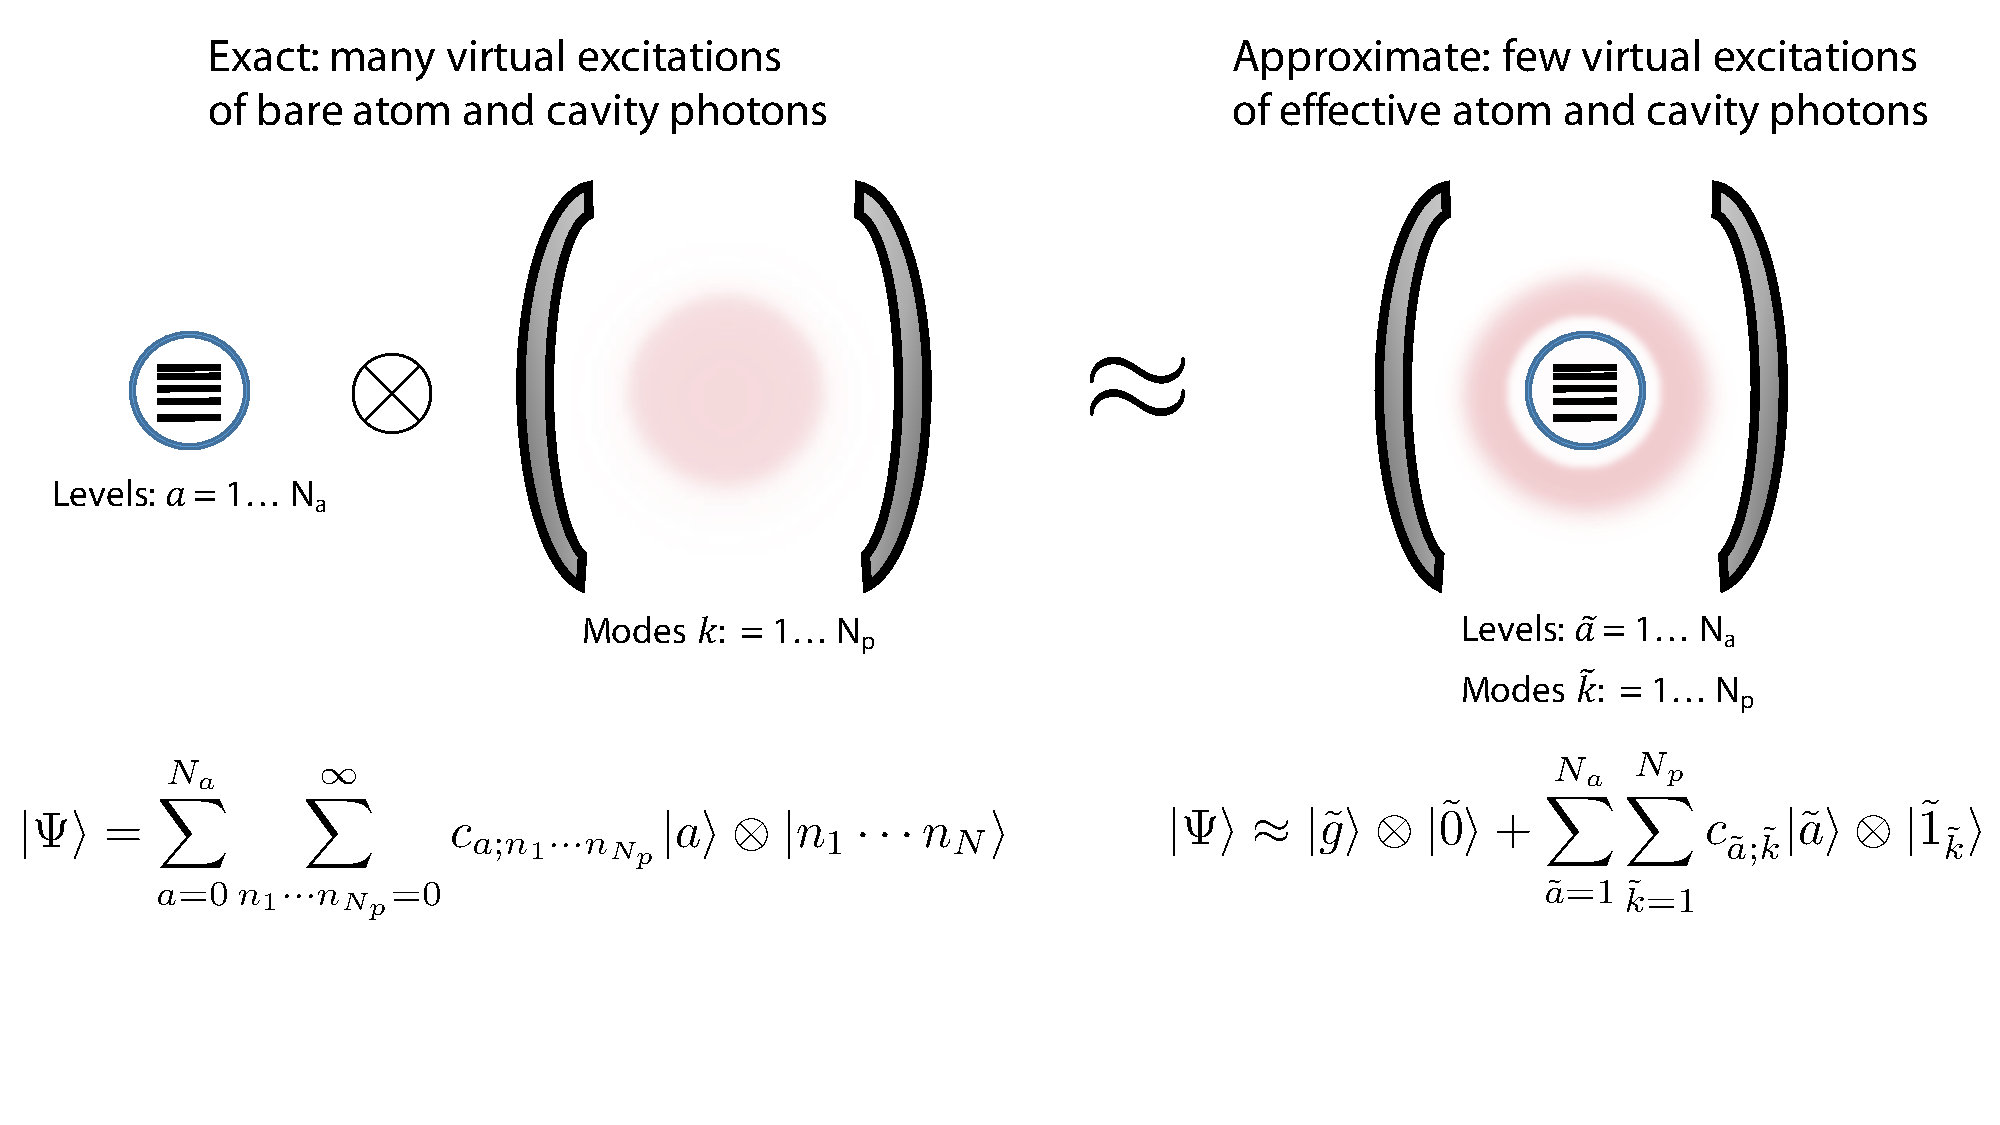
\includegraphics[width=18cm]{conceptfigure.pdf}
\caption{\textbf{Ground-state ansatz applied to matter in a cavity: effectively decoupled matter and photons.} .}
\label{fig:ansatz}
\end{figure*}

\subsection{Correlation corrections coming from virtual matter and photon quasiparticles}

\section{Application to a multi-level system coupled to a multi-mode cavity}

\section{Strategies for recovering the correlation energy}

\section{Outlook}



\section{Acknowledgements}
% Pri, Johannes: Please insert any other relevant acknowledgement information here!
N. R. and J. C. recognize the support of the DOE Computational Science Graduate Fellowship (CSGF) fellowship no.  DE-FG02-97ER25308. P. N. acknowledges start-up funding from the Harvard John A. Paulson School of Engineering and Applied Sciences. %The authors thank XXXX for helpful discussions. Tentatively Joel Yuen Zhou and Javier Aizpurua.

\bibliographystyle{apsrev4-1}
\bibliography{references}

\end{document}
